\hypertarget{md__home_yuan_Benchmarks_whisper_mnemosyne-gcc_usermode_library_pmalloc_include_alps_src_mainpage_mainpage}{}\section{A\+L\+P\+I\+Ni\+S\+M\+: Abstraction Layer for Programming Persistent Shared Memory   }\label{md__home_yuan_Benchmarks_whisper_mnemosyne-gcc_usermode_library_pmalloc_include_alps_src_mainpage_mainpage}
A\+L\+P\+I\+Ni\+SM provides a low-\/level abstraction layer that reliefs the user from the details of mapping, addressing, and allocating persistent shared memory (also known as fabric-\/attached memory). This layer can be used as a building block for building higher level abstractions and data structures such as heaps, logs, objects, etc.

 
\begin{DoxyImage}
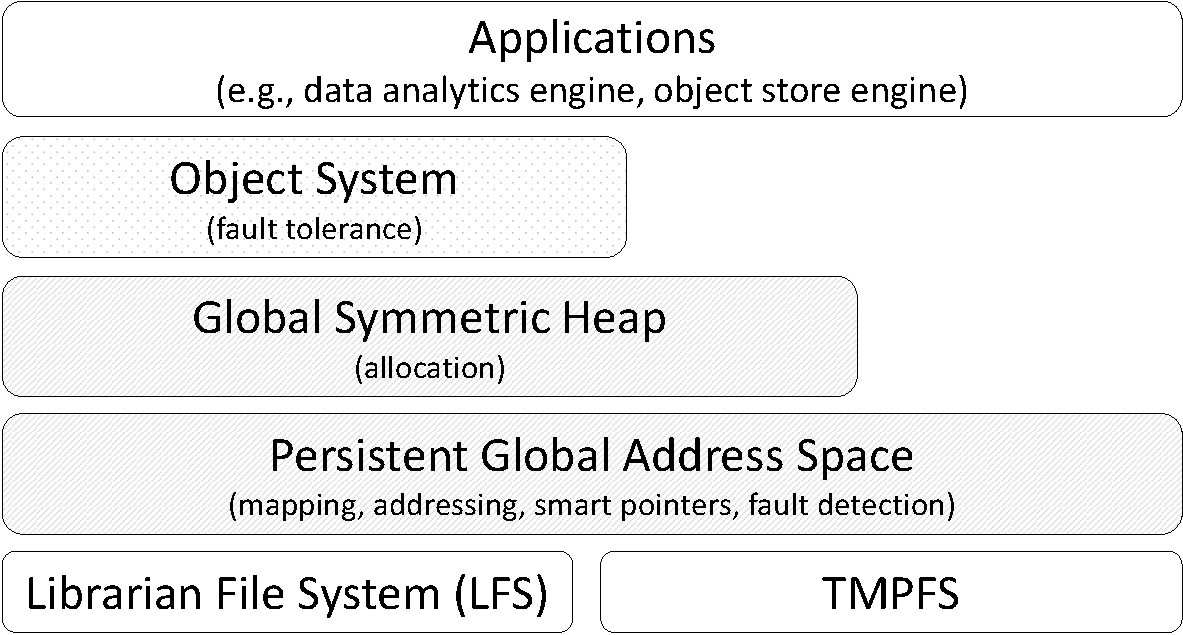
\includegraphics[width=10cm]{alps-layers}
\caption{A\+L\+P\+I\+Ni\+SM layers}
\end{DoxyImage}


Currently, we provide two layers (or A\+PI classes). First, a \hyperlink{md__home_yuan_Benchmarks_whisper_mnemosyne-gcc_usermode_library_pmalloc_include_alps_src_pegasus_pegasus_pegasuspage}{P\+Ersistent Global Address Space for Universal Sharing (P\+E\+G\+A\+S\+US)} layer provides a shared address space between multiple worker processes. Second, a Global Symmetric Heap layer for allocating variable-\/size chunks of shared persistent memory (a.\+k.\+a. fabric-\/attached memory).

The A\+P\+Is strive to be as generic as possible. Thus, we do not hardcode policy but instead seek providing generic mechanisms that can be used to support higher level policies.

\subsection*{Example Programs}

A\+L\+P\+I\+Ni\+SM comes with several samples in the {\ttfamily examples} directory.

\subsection*{This Document}

This document is written in Doxygen and maintained in the A\+L\+P\+I\+Ni\+SM git instance at\+:

\href{git://git-pa1.labs.hpecorp.net/ssftm/alps}{\tt git\+://git-\/pa1.labs.\+hpecorp.\+net/ssftm/alps}

\subsection*{Generating the documentation}

We include the A\+L\+P\+I\+Ni\+SM documentation as part of the source (as opposed to using a hosted wiki, such as the github wiki, as the definitive documentation) to enable the documentation to evolve along with the source code and be captured by revision control (currently git). This way the code automatically includes the version of the documentation that is relevant regardless of which version or release you have checked out or downloaded.

\begin{DoxyVerb} $ cd $ALPS/doc
 $ doxygen\end{DoxyVerb}


\subsection*{Reporting issues}

Please report feedback, including performance and correctness issues and extension requests, through the A\+L\+PS Jira instance\+:

\href{https://jira-pa1.labs.hpecorp.net/browse/ALPS/}{\tt https\+://jira-\/pa1.\+labs.\+hpecorp.\+net/browse/\+A\+L\+P\+S/}

\subsection*{Stable download locations}

The most recent version is published at\+: N/A

\subsection*{Contact information}

\begin{DoxyAuthor}{Author}
Haris Volos \href{mailto:haris.volos@hpe.com}{\tt haris.\+volos@hpe.\+com} 
\end{DoxyAuthor}
